\documentclass[10pt,letterpaper]{article}
\usepackage[utf8]{inputenc}
\usepackage{amsmath}
\usepackage{amsfonts}
\usepackage{amssymb}
\usepackage[margin=1in]{geometry}
\usepackage{graphicx}
\usepackage{sidecap}
\usepackage{float}
\title{\vspace{-4ex}Regression Variations\vspace{-3.5ex}}
\begin{document}
\newgeometry{top=0.75in,left=1in,right=1in,bottom=1.25in}
\maketitle
\vspace{-0.5em}
\begin{abstract}
A key feature of most machine learning models is their ability to learn and predict effectively; i.e. based on some given data points $X, Y$ that were generated non-randomly (with error given by a distribution), a well-formed model should be able to predict some reasonable pattern. To do this, we will often need to estimate some parameter $\theta$ that assigns weights to terms in our predicted function. The goal, then, is to choose the $\theta$ that leads to the minimum value of some error or loss function, and in this way minimize the error. This can be done in several ways, and a more formal and thorough treatment of this topic will be the subject of this paper.\\
\end{abstract}

\section{Gradient Descent}
First, we discuss the use of a tool that we will use often in calculating the minimum - gradient descent. We investigate several variations on its implementation, including analytic gradient descent, finite difference gradient descent, and Matlab's \texttt{fminunc}, which includes some variations such as adaptive step size, using a quadratic approximation instead of linear approximation, and using a 2-dimensional subspace to reduce computational complexity. First, we'll examine the analytic gradient descent, which relies on having an analytic expression for the gradient.

We'll refer to three example functions: the $n$-dimensional quadratic ``bowl'', $Q_n$, the $n$-dimensional inverted Gaussian (centered at $\mu = 0$, with $\Sigma = \mathbf I_n$), $N_n$, and the $n$-dimensional sum of sines, $S_n$. These are defined as follows (leaving off the normalization constant on the inverted Gaussian for simplicity):

\[ Q_n = \left\| \mathbf x \right\| ^2 \]

\[ N_n = -\exp{\left(-\dfrac{1}{2} \left\| \mathbf x \right\| ^2 \right)} \]

\[ S_n = \sum_{i=1}^n \sin(x_n) \]
Next, we benchmark the gradient descent variations on these two functions (seeding with an initial guess of $(1,1,\ldots)$):

\begin{table}[h]
\centering
\caption{Iterations (step = .1, threshold = .001)}
\begin{tabular}{r|ccc|ccc|ccc}
   & \multicolumn{3}{|c}{Analytic Gradient} & \multicolumn{3}{|c}{Finite Differences} & \multicolumn{3}{|c}{\texttt{fminunc}} \\
$n$& $Q_n$         & $N_n$        & $S_n$   & $Q_n$              & $N_n$   & $S_n$           & $Q_n$         & $N_n$        & $S_n$ \\\hline
2  & 16            & 33           & 46      & 16                 & 33      & 46              & 6             & 15           & 18    \\
5  & 18            & 60           & 50      & 18                 & 60      & 50              & 12            & 48           & 36    \\
20 & 21            &  1           & 57      & 21                 &  1      & 57              & 42            & 21           & 126   \\
100& 25            &  1           & 64      & 25                 &  1      & 64              & 202           & 101          & 606   
\end{tabular}
\end{table}

Focusing on just $S_n$, and leaving the step size, starting point, and threshold the same unless otherwise noted, we may also examine the effects of each variable (defaulting to $n=5$):

\begin{table}[h]
\centering
\caption{Examining the effect of other variables}
\begin{tabular}{cc|cc|cc}
\multicolumn{2}{c}{Step Size}& \multicolumn{2}{|c}{Starting Point} & \multicolumn{2}{|c}{Threshold} \\
$\Delta$  & Iterations        & $x_0$   & Iterations   & $\delta$  & Iterations     \\\hline
2.0       & 177               & 0.001   & 49           & 0.01      & 39     \\
1.0       & 5                 & 0.01    & 49           & 0.001     & 50     \\
0.1       & 61                & 0.1     & 50           & 0.0001    & 61     \\
0.01      & 503               & 1.0     & 61           & 0.00001   & 72  
\end{tabular}
\end{table}

We notice that the finite differences and analytic methods yield the exact same number of iterations for all functions. This can be explained by examining the diagonal of the Hessian matrix for each of the functions - in all cases, the values are small, indicating low curvature, and thus that the function can be well-approximated by the linear finite difference approximation. Therefore, when examining the effects of other variables, we only present the numbers using the finite-difference gradient (the analytic gradient produces identical numbers).

We may draw a few conclusions by examining the effects of other variables. As we decrease the step size, it takes longer to converge. However, increasing the step size beyond 1 causes the iteration to overshoot, resulting in an overall higher number of required iterations. Moving the starting point further from the minimum increases the number of iterations, but only slightly, because the gradient increases, which increases the step size proportionally. Finally, requiring a stricter convergence criteria via a smaller threshold increases the number of iterations, but only by a constant amount, because the gradient again ensures the step size is in proportion to the distance from the minimum.

By plotting the difference between the finite differences approximation, we can see the accuracy achieved. Here, we again use $\delta = .01$. Figures \ref{fig:gradDifQ} through \ref{fig:gradDifS} are plots of $(\nabla f(\mathbf{x}) - \tilde{\nabla} f(\mathbf{x}))/f(\mathbf{x})$ for $x=(0,1)$.

\begin{figure}[!htb]
\minipage{0.32\textwidth}
  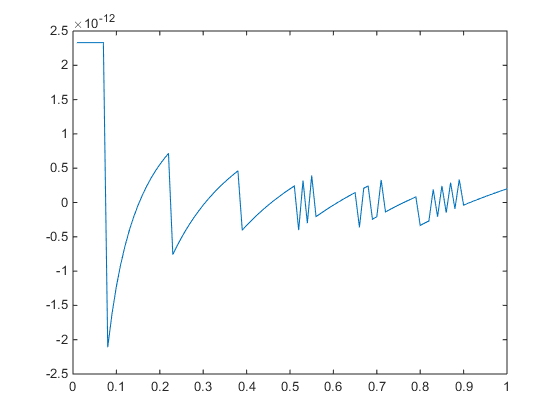
\includegraphics[width=\linewidth]{figures/gradDifQ.png}
  \caption{$Q_1$, scale of $10^{-12}$}\label{fig:gradDifQ}
\endminipage\hfill
\minipage{0.32\textwidth}
  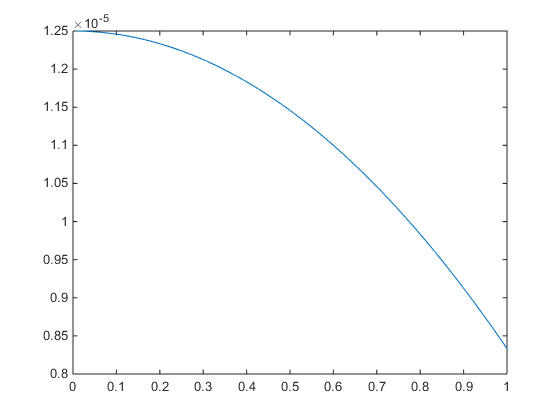
\includegraphics[width=\linewidth]{figures/gradDifN.png}
  \caption{$N_1$, scale of $10^{-5}$}\label{fig:gradDifN}
\endminipage\hfill
\minipage{0.32\textwidth}
  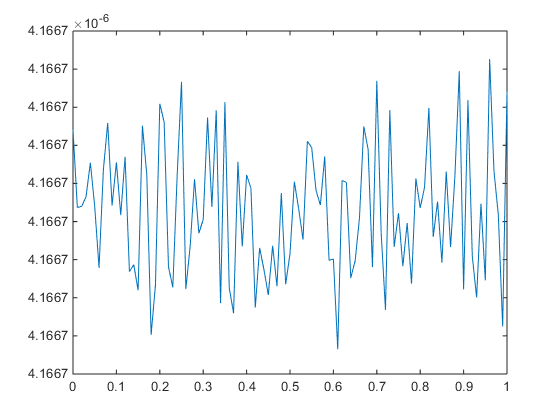
\includegraphics[width=\linewidth]{figures/gradDifS.png}
  \caption{$S_1$, scale of $10^{-6}$}\label{fig:gradDifS}
\endminipage
\end{figure}

Given the scales of the plots, it is clear that the finite differences method is quite accurate for these functions over these distance scales. As noted, this is generally true when the diagonal entries of the Hessian matrix are small.

\section{Some Simple Regression}
Now that we've established gradient descent as a reliable tool to help us calculate minima, we can benchmark it by applying it directly through performing basis function regression on some given sample data points. Given, say, $10$ data points $X = x^{(1:10)}$ that are generated from a noisy distribution around $y = \sin(2\pi x)$, we'll try to estimate the generating function based on (a) the values at the data points $Y = y^{(1:10)}$ and (b) a basis set of functions.

Our ultimate goal is the minimize the sum of the squared errors of each of our proposed predictions, or $\text{SSE}(\theta)$, which is equal to
\[ \text{SSE}(\theta) = \sum_{i=1}^n (\theta^\intercal\phi(x^{(i)}) - y^{(i)})^2 \]

We can begin by considering a simple polynomial basis; i.e. $\phi(x) = [1, x, x^2, \ldots , x^M]$ where $M$ is the degree of the polynomial we are considering. We wish to minimize our parameter $\theta$, which has a well-known analytic solution:
\[ \theta = (\Phi^\intercal\Phi)^{-1}\Phi^\intercal y \]
given that $\Phi = \phi(x)$ generally, and specifically
\[ \Phi = \left( \begin{array}{cccc}
 1 &  x^{(1)} & \ldots & (x^{(1)})^M \\
 \vdots & \vdots & & \vdots \\
 1 &  x^{(n)} & \ldots & (x^{(n)})^M \end{array} \right) \]
for this polynomial basis. We can easily test this by plotting our data $(X, Y)$ with our learned model $\theta^\intercal\phi(X)$ for varying values of $M$, shown in figures \ref{fig:basism1} through \ref{fig:basism9}.

\begin{figure}[h]
\minipage{0.33\textwidth}
  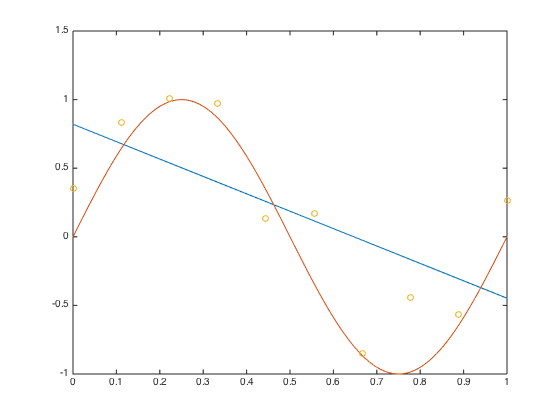
\includegraphics[width=\linewidth]{figures/basism1.png}
  \caption{$M = 1$}\label{fig:basism1}
\endminipage\hfill
\minipage{0.33\textwidth}
  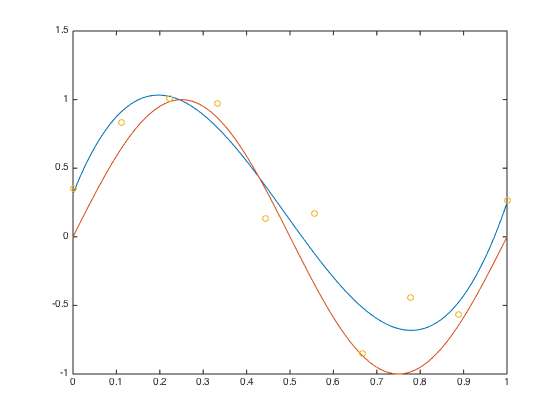
\includegraphics[width=\linewidth]{figures/basism3.png}
  \caption{$M = 3$}\label{fig:basism3}
\endminipage\hfill
\minipage{0.33\textwidth}
  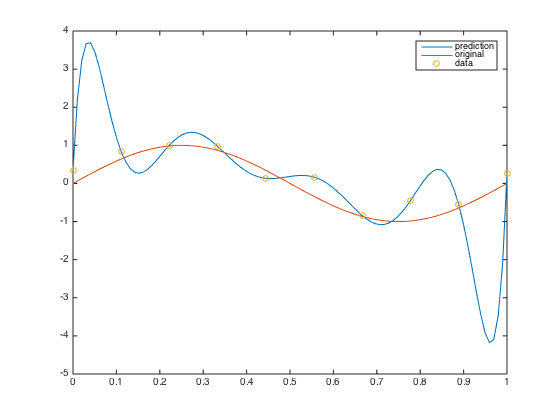
\includegraphics[width=\linewidth]{figures/basism9.png}
  \caption{$M = 9$}\label{fig:basism9}
\endminipage
\end{figure}
We note that we can't have $M > 9$, or else we have too many parameters to adjust for the data points that we have. The reason the formula breaks down is that $\Phi^\intercal\Phi$ is no longer full rank, which means we can no longer simply take the inverse to find $\theta$. In other words, there are now many (in fact, infinitely many) sets of parameters that would perfectly fit the criteria. We can adjust for this using the \textit{Moore-Penrose inverse} which pulls the $\theta$ from the list with the smallest norm. We will not address this in detail here.

From figure \ref{fig:basism9}, it's also clear that when $M$ is too high, we begin to overfit our data, even though the training error here is $0$. We will come back to this problem later, when we deal with regularization.

At the moment, however, we can generalize our basis functions to more than simply polynomials in $x$. In this way, we can introduce trigonometric bases, exponential bases, etc. to give us more flexibility in choosing the parameter $\theta$. 
We can minimize this by using gradient descent, which we discussed earlier. We can then confirm our calculations analytically by computing the derivative of $\text{SSE}(\theta)$:
\[ \frac{\partial}{\partial\theta}\Big(\sum_{i=1}^n (\theta^\intercal\phi(x^{(i)}) - y^{(i)})^2\Big) = 2\sum_{i=1}^n \phi(x^{(i)})(\theta^\intercal\phi(x^{(i)}) - y^{(i)}) \]
Plugging in our optimal $\theta$ into this formula and calculating the numerical gradient with a $\delta$ of 0.00001, we obtain the following results for our derivative:
\begin{table}[h]
\centering
\caption{Examining the the numerical vs. analytic derivatives}
\begin{tabular}{c|c|c}
$M$& $\lVert\nabla\text{SSE}(\theta)\rVert$ (numerical) & $d\text{SSE} (\theta)/d\theta$ (analytic)\\\hline
0       &  $2.1067\cdot10^{-12}$  & $1.6653\cdot10^{-16}$   \\
1       & $2.1165\cdot10^{-12}$  & $1.0335\cdot10^{-14}$ \\
3       & $1.7099\cdot10^{-11}$ & $7.9814\cdot10^{-10}$  \\
9      &   $7.9814\cdot 10^{-10}$    & $-1.6414\cdot 10^{-07}$
\end{tabular}
\end{table}

%Now let us try minimizing the $\theta$ with gradient descent, to find a minimum for the loss so that our $\theta$ is optimal. We obtain the following results:


In addition, it is tempting to fit this data set by using $\phi_1(x) = \sin(2\pi x), \ldots , \phi_M(2\pi Mx)$ as our basis set of functions. If we use these, our plots in figures \ref{fig:sin1} to \ref{fig:sin6} look much closer to the original function. However, if we didn't already know anything about the data, guessing a basis of only sinusoidal functions comes with a serious disadvantage. It guarantees that all our generated $\theta^\intercal\phi(x)$ will be periodic in nature, when the actual data/observations really aren't. This can cause unnecessarily varying, and potentially completely incorrect, data to be predicted.\\
\begin{figure}[h!]
\minipage{0.33\textwidth}
  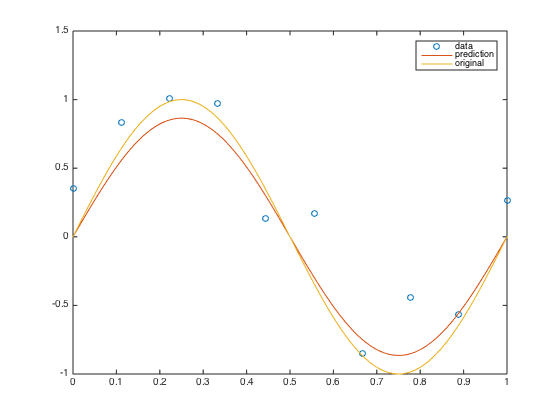
\includegraphics[width=\linewidth]{figures/sin1.png}
  \caption{$M = 1$}\label{fig:sin1}
\endminipage\hfill
\minipage{0.33\textwidth}
  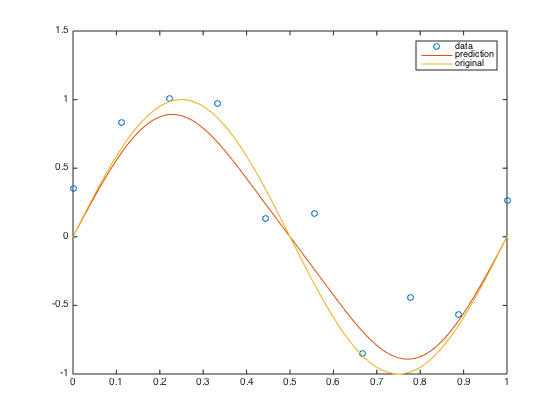
\includegraphics[width=\linewidth]{figures/sin3.png}
  \caption{$M = 3$}\label{fig:sin3}
\endminipage\hfill
\minipage{0.33\textwidth}
  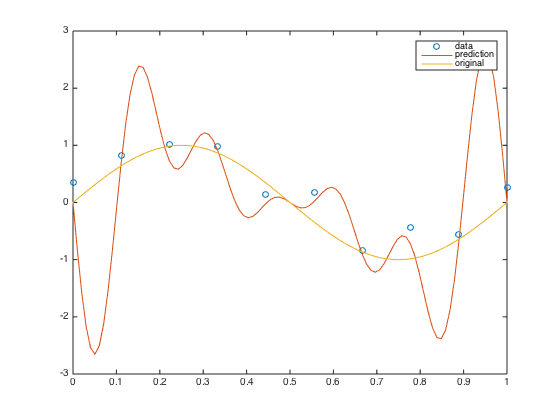
\includegraphics[width=\linewidth]{figures/sin6.png}
  \caption{$M = 6$}\label{fig:sin6}
\endminipage\hfill
\end{figure}



\section{Ridge Regression}

Recall that earlier, we had the problem that having too high of an $M$ could cause overfitting to the training data. Now we will examine ridge regression, which is a form of regression that attempts to minimize the coefficients of $\Theta$; this will reduce the magnitudes of the coefficients of a high-order polynomial to more reasonable sizes. It does this by imposing a penalty, $\lambda$, on the Euclidean (squared) norm of the coefficients of $\Theta$:
$$\theta_{\text{ridge}} = \text{argmin}_\theta\sum_{i=0}^n(y^{(i)} - \theta^\intercal\phi(x^{(i)}))^2 + \lambda\lVert\theta\rVert^2$$
The fact that we impose a penalty on the Euclidean norm is a direct result of considering the noise as a Gaussian. Considering the noise as a Laplacian distribution leads to imposing a penalty on the absolute value norm, while other noise distributions lead to yet more functions of $\theta$ to apply the penalty to. The first term is simply $\text{SSE}(\theta)$, so it isn't surprising that the analytic solution to this minimization is similar to that of just $\text{SSE}(\theta)$; it's given by
\[ \theta = (\Phi^\intercal \Phi + \lambda \mathbf{I})^{-1}\Phi^\intercal y \]
where $\Phi = \phi(X)$. We then have the predictor function given by $\phi$ weighted by $\theta$, eg, we would predict $y_{predicted} = \theta^\intercal \phi(x')$.
\begin{figure}[!htb]
\minipage{0.49\textwidth}
  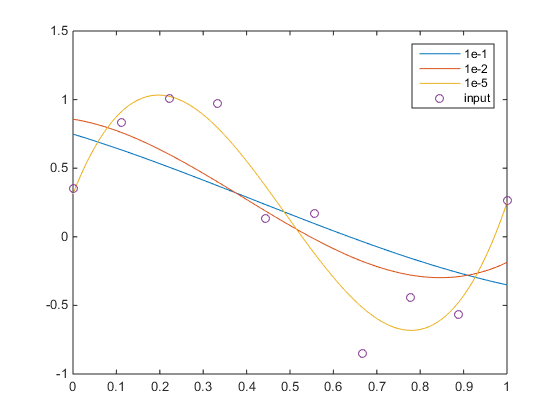
\includegraphics[width=\linewidth]{figures/M3.png}
  \caption{$M=3$}\label{fig:M3}
\endminipage\hfill
\minipage{0.49\textwidth}
  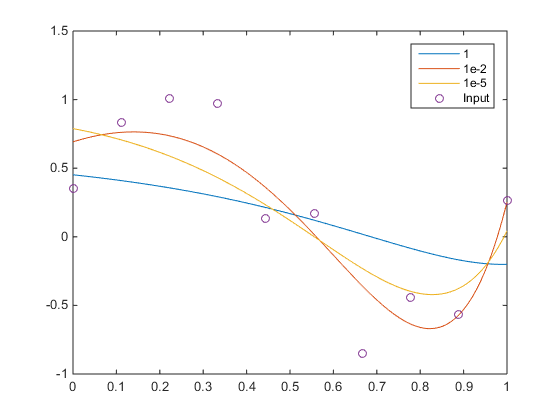
\includegraphics[width=\linewidth]{figures/M7.png}
  \caption{$M=7$}\label{fig:M7}
\endminipage
\end{figure}
We can see the effect $\lambda$ has on the result by examining a few values of $\lambda$ for the same dataset used previously (generated from $\sin(2\pi x)$).

The effect of $\lambda$ is clear in Figures \ref{fig:M3} and \ref{fig:M7}, where higher values of $\lambda$ lead to flatter, smoother approximations. As $M$ increases (especially relative to $n$), the values in $\theta$ begin rising enormously, but adding the $\lambda$ factor helps to keep them under control. For example, in this example with $M=7$, $\max \theta_i = 1595.9$ for $\lambda = 0$, but for $\lambda = .01$, $\max \theta_i = 1.7781$, a much more reasonable value, and far more likely to approximate the truth accurately. In particular, Figure 1.8 in Bishop nicely summarizes the assistance $\lambda$ gives in generalizing $\theta$.

\begin{figure}[!h]
\begin{center}
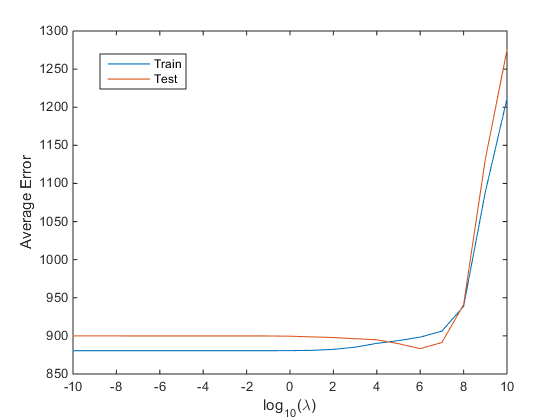
\includegraphics[width=4in]{figures/blogData.png}
\caption{Effect of $\lambda$ on training and test errors.}\label{fig:blogData}
\end{center}
\end{figure}
Applying ridge regression to a real-world data set, we can also observe the effects of $\lambda$. Here, we apply ridge regression to a dataset regarding blogs, where the $x$ vector contains 280 metrics for each blog post, and $y$ is the number of comments in the first 24 hours. We can see the effect $\lambda$ has on the training error and testing error in figure \ref{fig:blogData}. From this, we conclude that $\lambda=10^8$ is the approximately optimal value of $\lambda$ for this problem.\\

\section{LAD}
All this time, in applying various regression techniques, we have been assuming the use of our $\text{SSE}(\theta)$ function to minimize our $\theta$ (with the possible addition of a regularization term, e.g. $\lambda\lVert\theta\rVert^2$ in ridge regression). We see that a squared regularization term comes naturally in the context of Gaussians; if instead we used a linear loss based on the non-square norm (using $\lambda\lVert\theta\rVert$), we are pulling from a Laplace distribution - this regularization is commonly termed LASSO.

However, in our case, we'll leave the regularization term alone and instead investigate changes in our $\text{SSE}(\theta)$ term. Here we can use a linear model instead of a quadratic one, so that we sum our absolute errors to obtain our residual error. This method is called ``LAD'' (least absolute deviations):

$$\theta_{\text{LAD}} = \text{argmin}_\theta\sum_{i=0}^n|y^{(i)} - \theta^\intercal\phi(x^{(i)})| + \lambda\lVert\theta\rVert^2$$

Note that we are no longer minimizing anything similar to $\text{SSE}(\theta)$. As this problem has no simple analytical solution, we can again make use of gradient descent, this time to solve for our parameter $\theta$, for the same varying values of lambda we used above in normal ridge regression:

The results are expected; in general, we find that least absolute deviations is more robust than least squares regression, as it is less susceptible to outliers in the dataset. This is an especially important point - if we don't wish for our model to give heavier weight to outliers, then LAD is the better choice.

Ridge regression, however, produces results that are more stable, with the derivative falling off more slowly and the solution being unique. It has the advantage of having a simple, standard and well-known analytic solution that is more easily implemented. In addition, if we want outliers to have more effect on our model, then we should choose ridge regression. The choice of regression function is entirely up to the characterics of the data we would like to model.

\end{document}













